% !TEX root = Master.tex

\begin{figure}[H]
\centering
  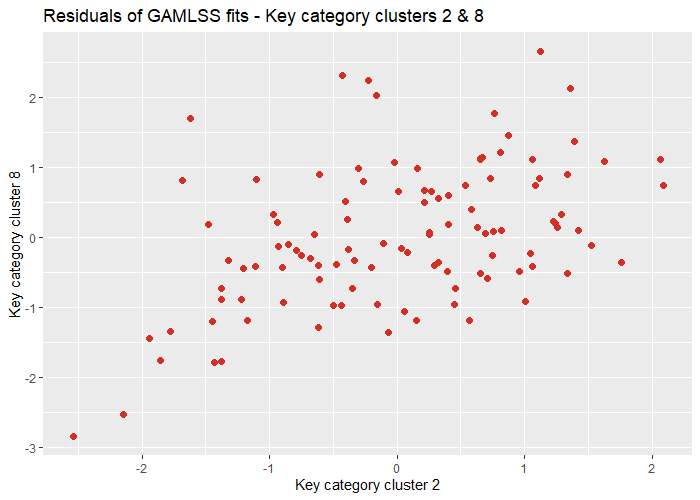
\includegraphics[width=0.45\linewidth]{figures/scatter_res_kcc_28.png}
  \caption{Scatterplot of estimated residuals of GAMLSS fits for key category clusters 2 \& 8}
  \label{fig:scatter_res_kcc_28}
\end{figure}



\inputRoutput[caption={Summary of GJRM fit on key category clusters 2 \& 8},numbers=left,numberstyle=\tiny, label=output:summary_kcc_28]{summary_kcc_28.txt}



\begin{figure}[H]
\centering
  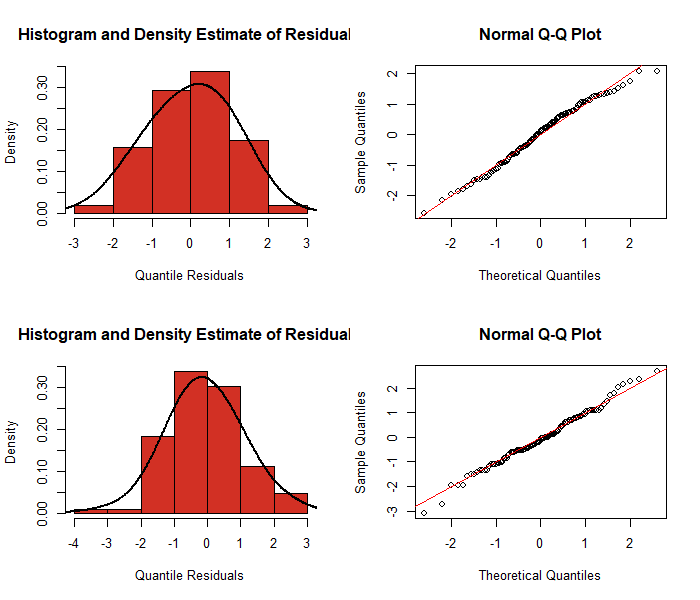
\includegraphics[width=0.95\linewidth]{figures/res_hist_qqplot_28.png}
  \caption{Diagnostic plots of quantile residuals based on \ac{GJRM} models for key category clusters 2 \& 8}
  \label{fig:res_hist_qqplot_28}
\end{figure}


\begin{figure}[H]
\centering
  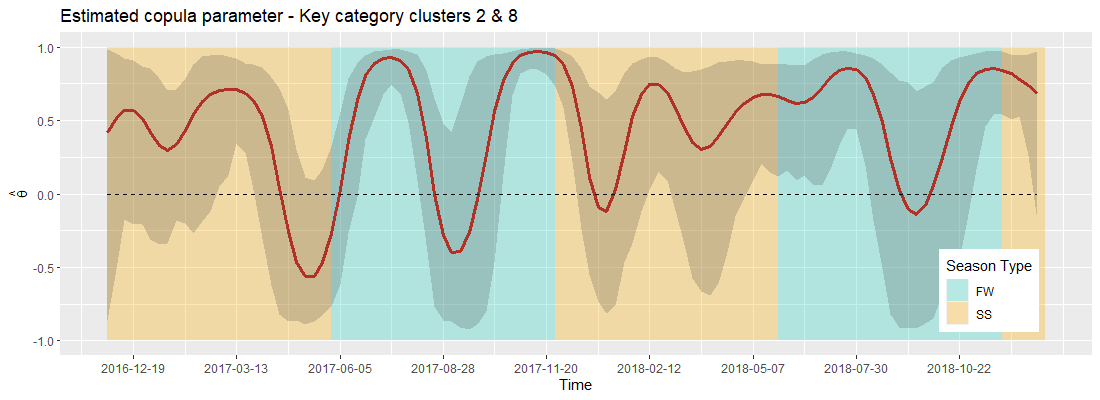
\includegraphics[width=0.95\linewidth]{figures/estimated_theta_kcc_28.png}
  \caption{Estimated copula parameter over time from a \ac{GJRM} t-copula model with normal margins for key category clusters 2 \& 8 with 95\% confidence bands}
  \label{fig:estimated_theta_kcc_28}
\end{figure}




\begin{figure}[H]
\centering
  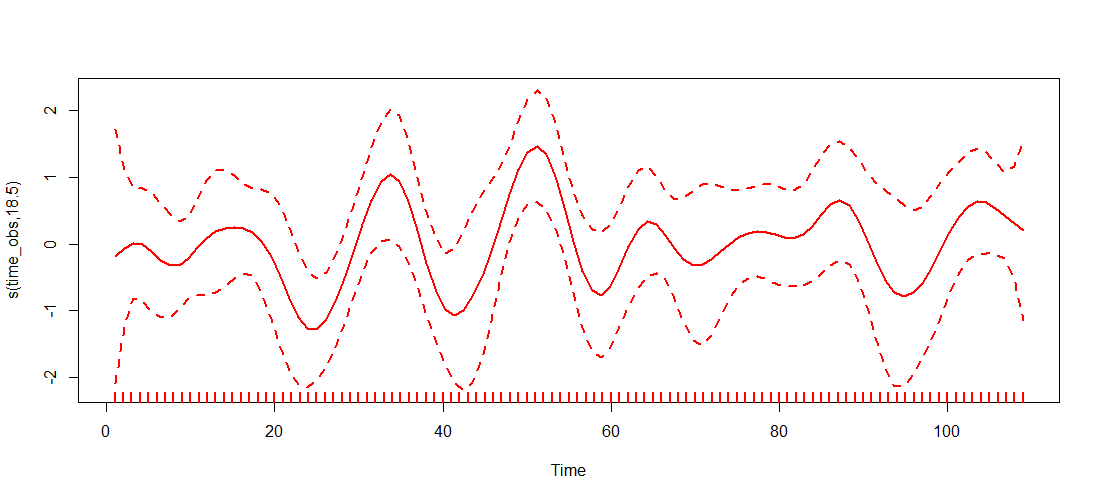
\includegraphics[width=0.95\linewidth]{figures/time_effect_on_theta_28.png}
  \caption{Estimated Smooth effect of time on the copula parameter $\theta$ with 95\% confidence bands for key category clusters 2 \& 8}
  \label{fig:time_effect_on_theta_28}
\end{figure}











%On this \ac{KCC} pair, the \ac{GJRM} approach is not as favorable as in the pair KCC 2 \& KCC 6, though it might be considered acceptable (\autoref{fig:margin_estimates_kcc_28}).  \\
%
%\begin{figure}[H]
%\centering
%  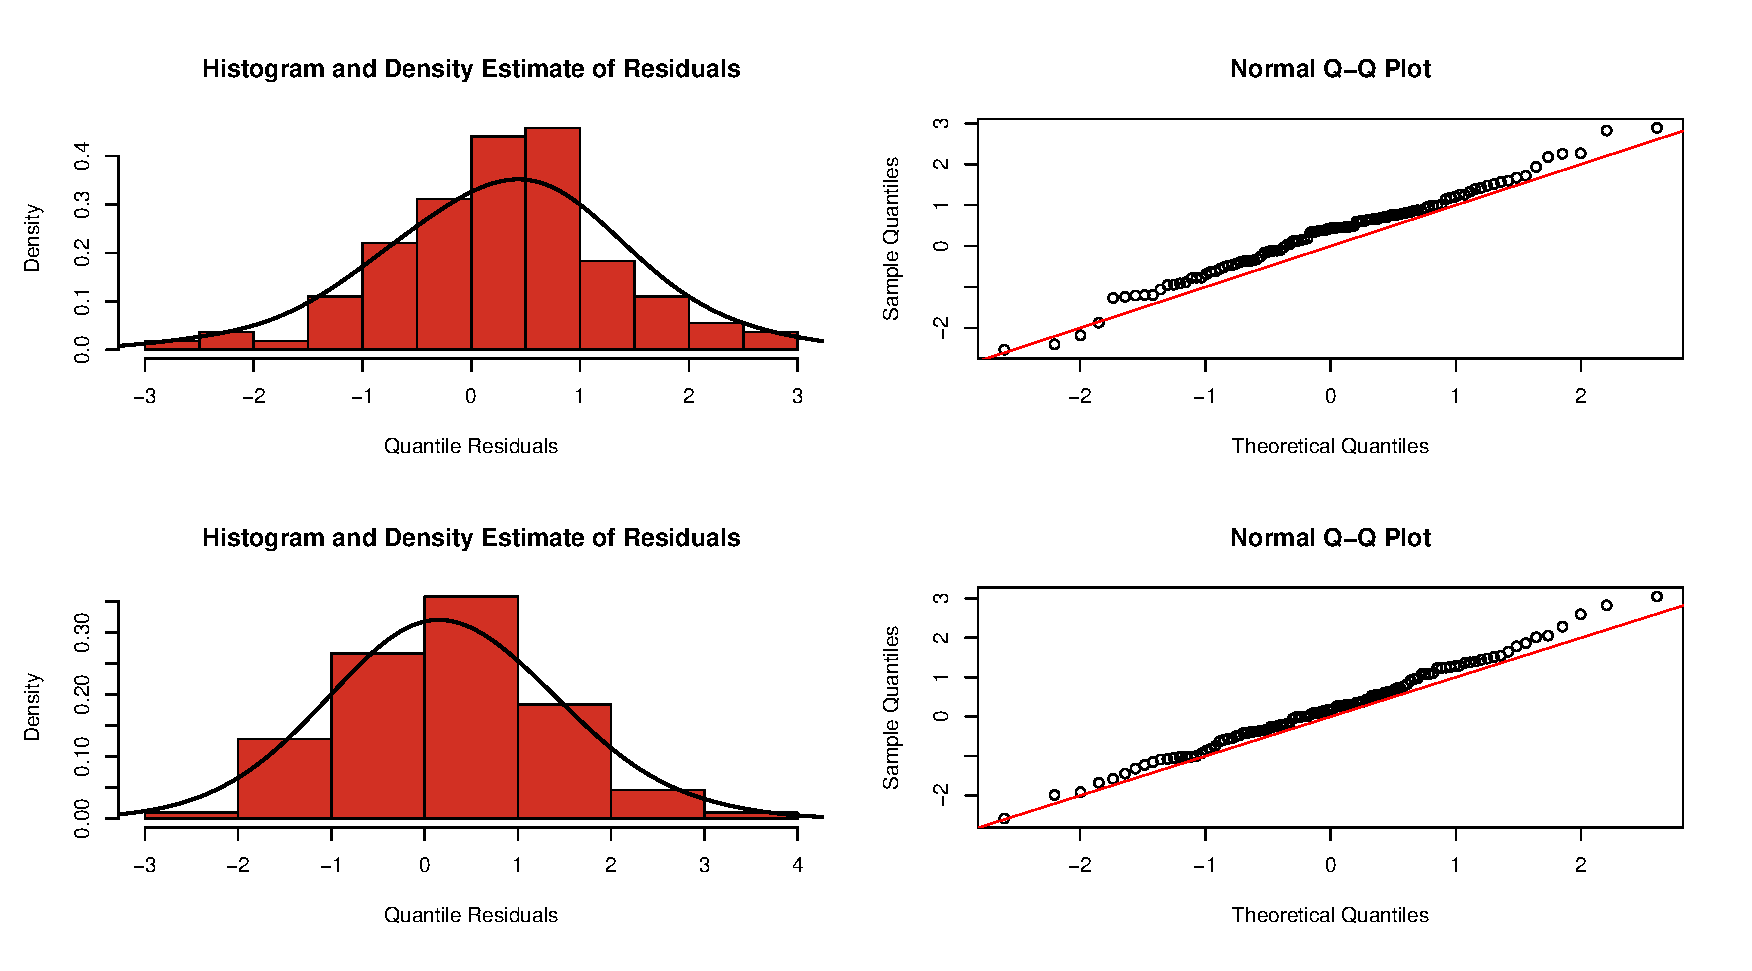
\includegraphics[width=0.9\linewidth]{figures/margin_estimates_kcc_28.eps}
%  \caption{Estimation diagnostics for the response marginals KCC 2 \& KCC 8; \ac{GJRM} approach}
%  \label{fig:margin_estimates_kcc_28}
%\end{figure}
%
%This circumstance is reflected within the comparison of the "gamCopula" estimated dependence measures. The overall similarity between the two lines in \autoref{fig:copula_parameters_28}, which depict the time-dependent correlation parameters of this pair, is given. However, the details reveal that there are severe differences between the estimation methods. As the gamCopula approach yields converge in contrast to the \ac{GJRM} method, it might be preferential. Nevertheless, the results should be treated with adequate caution.
%
%\begin{figure}[H]
%\centering
%  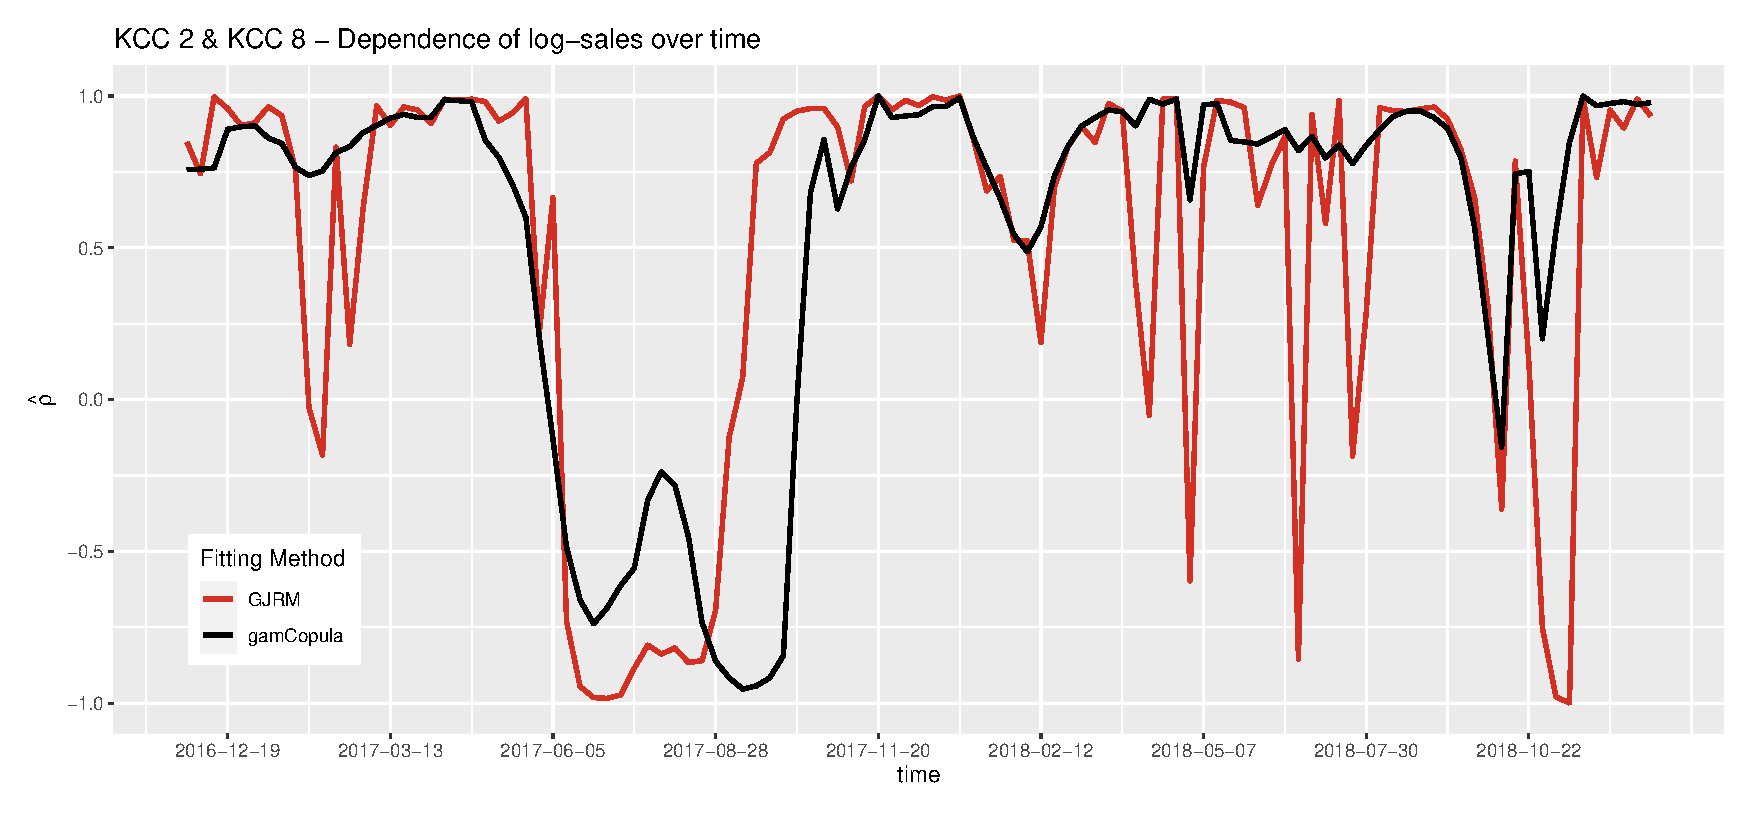
\includegraphics[width=0.9\linewidth]{figures/copula_parameters_28.eps}
%  \caption{Estimated time-varying Pearson's correlation coefficients for the pair KCC 2 \& KCC 8}
%  \label{fig:copula_parameters_28}
%\end{figure}
%
%
%The stretched sign change of the correlation over time happens, just like in the previous pair, from June to August 2017. The curves here are surprisingly different in terms of their stability. The gamCopula method seems to have a more stable course compared to the \ac{GJRM} approach. The red line in \autoref{fig:copula_parameters_28} appears very sensitive in very short time intervals.



